
\chapter{Introduction to Differential Calculus}\label{Chapter:Calculus}


\section{Limits \& Continuity}\label{Section:LimitsContinuity}

Informally, the limit of a function $\limit{x}{a} f(x)=L$ (if it exists) is a number $L$ such that when $f(x)$ get's closer and closer to $a$, $f(x)$ gets closer and closer to $L$. \\

Consider the function $f(x)=\frac{x^2-1}{x-1}$, what happens as $x$ get's closer and closer to 1?

$$
\begin{array}{|c|c|}
\hline
x & f(x)\\
\hline
1.1 & 2.1\\
1.01 & 2.01\\
1.001 & 2.001\\
.9 & 1.9\\
.99&1.99\\
.999 & 1.999\\
\hline
\end{array}$$

You can test and see these values here: \url{https://www.desmos.com/calculator/w3ycpf3mv4}.  It certainly seems as if $x$ gets closer and closer to $1$, $f(x)$ approaches the value $2$.  Why couldn't we just plug in 1?  Because if we did we would get $f(1)``="\frac{1^2-1}{1-1}``="\frac{0}{0}$ which is undefined.  Recall that $1$ would not be a part of the domain of $f(x)$.  This, in fact, is the whole point of limits, the entire reason they exist, is in order to give values to things like $f(1)$ which are not defined.\\

The left and right limits of a function are values the function approaches as $x$ $a$ from the left or the right, so as we see above, they both (the black and orange dots in the linked graph) both approach the same value.  So:

\begin{itemize}
\item $\limit{x}{1^-}\frac{x^2-1}{x-1}=2$.
\item $\limit{x}{1^+}\frac{x^2-1}{x-1}=2$
\item $\limit{x}{1}\frac{x^2-1}{x-1}=2$
\item $f(1)$ is undefined.
\end{itemize}

So looking at this graph:
$$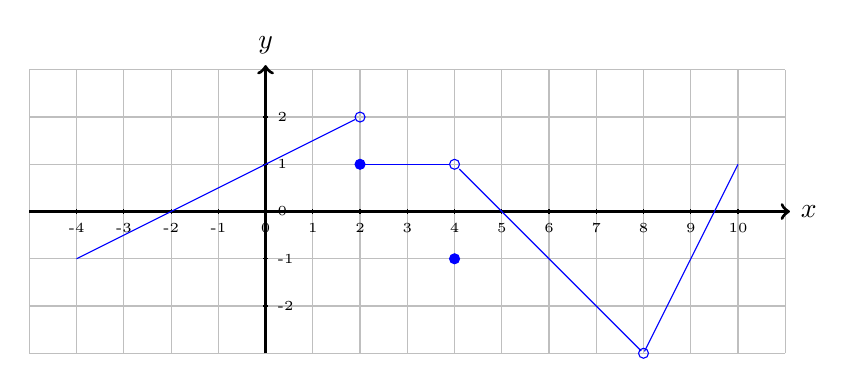
\begin{tikzpicture}[scale=.6][domain=-5:11]
    \draw[gray!50, thin, step=1] (-5,-3) grid (11,3);
    \draw[very thick,->] (-5,0) -- (11.1,0) node[right] {$x$};
    \draw[very thick,->] (0,-3) -- (0,3.1) node[above] {$y$};

    \foreach \x in {-4,...,10} \draw (\x,0.05) -- (\x,-0.05) node[below] {\tiny\x};
    \foreach \y in {-2,...,2} \draw (-0.05,\y) -- (0.05,\y) node[right] {\tiny\y};

    \draw[blue] (2,2) circle (3pt);
    \draw[ blue, fill] (2,1) circle (3pt);
    \draw[blue] (4,1) circle (3pt);
    \draw[fill, blue] (4,-1) circle (3pt);
    \draw[blue] (8,-3) circle (3pt);


  \draw[scale=1,domain=-4:1.9,smooth,variable=\x,blue] plot ({\x},{.5*\x+1});
  \draw[scale=1,domain=2.1:3.9,smooth,variable=\x,blue] plot ({\x},{1});
  \draw[scale=1,domain=4.1:7.95,smooth,variable=\x,blue] plot ({\x},{-1*\x+5});
  \draw[scale=1,domain=8.02:10,smooth,variable=\x,blue] plot ({\x},{2*\x-19});


\end{tikzpicture}$$

For $x=2,4,6,8$, find the left and right limits, the limit, and the value of the function.  See if you understand why the following are true:

\begin{itemize}
\item $\limit{x}{2^-}f(x)=2$, as we approach $x$ from the left, this is what $f(x)$ approaches.
\item $\limit{x}{2^+}f(x)=1$, as we approach $x$ from the right, this is what $f(x)$ approaches.
\item $\limit{x}{2}f(x)$ is undefined, there is no single number that $f(x)$ get's closer to, so there is no limit.
\item $f(2)=1$, that's the actual value of $f(2)$.
\end{itemize}

Similarly, we should see:

\begin{itemize}
\item $\limit{x}{4^-}f(x)=1$.
\item $\limit{x}{4^+}f(x)=1$.
\item $\limit{x}{4}f(x)=1$.
\item $f(4)=-1$.
\item $\limit{x}{6^-}f(x)=-1$.
\item $\limit{x}{6^+}f(x)=-1$.
\item $\limit{x}{6}f(x)=-1$.
\item $f(6)=-1$.
\item $\limit{x}{8^-}f(x)=-3$.
\item $\limit{x}{8^+}f(x)=-3$.
\item $\limit{x}{8}f(x)=-3$.
\item $f(8)$ is undefined.
\end{itemize}

A great shorthand for determining when there is or isn't a limit is: ``$\limit{x}{a}f(x)=L$ and exists if and only if $\limit{x}{a^-}f(x)=L$ and $\limit{x}{a^+}f(x)=L$"

\subsection{Continuity}

I'm not going to overblow continuity with to much verbiage here since we intuitive understand what it means to be continuous, it just means that all the points ``connect".  So what does tat mean for us above?  Out of the values $x=2,4,6,8$, where is $x$ continuous?

It seems like it's only 6 where it's continuous.  2 and 4 have jump discontinuities, and $f(x)$ isn't even defined at $x=8$ so how could it be continuous there?  So the definition of continuous is as intuitive as we would like:\\

$f(x)$ is continuous at $a$ if and only of $f(a)=\limit{x}{a} f(x)$.  So as in above, out of the 4 points we looked at, $x=6$ is the only place where everything ``behaves properly" and we get continuity.




\section{Average rates of change}\label{Section:AvgRoC}

Consider a rocket that is launched into the air and has height $f(x)=-5x^2+20x$ meters in $x$ seconds. \url{https://www.desmos.com/calculator/1rwsdsbcm9}. How fast is the rocket traveling when it's launched ($x=0$ seconds)?\\

Turns out, it's not so easy to think about what this is, we don't typically think about speeds in terms of instantaneous action.  Our methods of measuring speed reflects this, it's always stuff like meters \textbf{ PER SECOND}, miles \textbf{ PER HOUR}, in other words speed is some change in distance \textbf{ OVER TIME} and that period of time is not typically 0.\\

So what now?  Lets start by asking an easier question, what is the average speed of the rocket over the first 3 seconds?\\

It's best in a scenario like this to NOT overthink the underlying problem.  At 0 seconds, you're $f(0)=-5(0)^2+20(0)=0$ meters off the ground.  After 3 seconds you are $f(3)=-5(3^2)+20(3)=15$ meters off the ground.  So you rose by 15 meters in 3 seconds?  You're aveerage speed must be 5 meters per second. \url{https://www.desmos.com/calculator/6k61owwnrd}.\\

In fact:  \textbf{ The average rate of change of a function $f(x)$ over the interval $[a,b]$ is $m=\frac{f(b)-f(a)}{b-a}$.}  This is just the slope of the line connecting $(a,f(a))$ and $(b,f(b))$.\\

Following this idea, the average velocity of our rocket over the 1st 2 seconds is: $m=\frac{f(2)-f(0)}{2-0}=\frac{20}{2}=10$ meters per second. \url{https://www.desmos.com/calculator/ihauynuflo}\\

The average velocity of our rocket over the 1st second is: $m=\frac{f(1)-f(0)}{1-0}=\frac{15}{1}=15$ meters per second. \url{https://www.desmos.com/calculator/jce0fd1bsr}\\

The average velocity of our rocket over the 1st half second is: $m=\frac{f(.5)-f(0)}{.5-0}=\frac{8.75}{.5}=17.5$ meters per second. \url{https://www.desmos.com/calculator/xpxlltf8f5}\\

The average velocity of our rocket over the 1st quarter second is: $m=\frac{f(.25)-f(0)}{.25-0}=\frac{4.6875}{.25}=18.75$ meters per second. \url{https://www.desmos.com/calculator/74kpvz17c5}\\

The average velocity of our rocket over the 1st tenth of a second is: $m=\frac{f(.1)-f(0)}{.1-0}=\frac{1.95}{.1}=19.5$ meters per second. \url{https://www.desmos.com/calculator/qyvtzmyg8k}\\

The average velocity of our rocket over the 1st hundreth of a second is: $m=\frac{f(.01)-f(0)}{.01-0}=\frac{.1995}{.1}=19.95$ meters per second. \url{https://www.desmos.com/calculator/hrawtifwdw}\\


And it does seem like these numbers are getting closer and closer to 20 meters per second as $b$ gets closer to 0.  But if I plug in $0$ for $b$, I get an undefined $0/0$ fraction.  Oh, if only there were some concept in mathematics to describe the values of a function as your inputs slowly approach a given value.........

\section{The Derivative as a Limit}\label{Section:DefofDerivative}

Let's be a bit more general for just a moment, suppose that we had a function $f(x)$ and we wanted to know what the instantaneous rate of change of a function was at some given $x$.  Well, if we stepped forward by $h$ units, we could measure the average rate of change of $f(x)$ over $[x, x+h]$, this would be $$\frac{f(x+h)-f(x)}{x+h-x}=\frac{f(x+h)-f(x)}{h}.$$

What we just observed is that if we let $h$ converge towards 0, that it seems as if our quotient also converges to some value.  This value is the derivative of $f(x)$ at $x$ and is denoted and defined as $$f'(x)=\limit{h}{0}\frac{f(x+h)-f(x)}{h}.$$

So how does this play out given our rocket?  Well:

\begin{eqnarray*}
f'(x)&=&\limit{h}{0}\frac{f(x+h)-f(x)}{h}\\
&=&\limit{h}{0} \frac{-5(x+h)^2+20(x+h)-(-5x^2+20x)}{h}\\
&=&\limit{h}{0}\frac{-5x^2-10xh-5h^2+20x+20h+5x^2-20x}{h}\\
&=&\limit{h}{0}\frac{-10xh-5h^2+20h}{h}\\
&=&\limit{h}{0}\frac{(-10x-5h+20)h}{h}\\
&=&\limit{h}{0} -10x-5h+20\\
&=&-10x+20.
\end{eqnarray*}


So this means that in $0$ seconds, the change in the height was $f'(0)=-10(0)+20=20$ meters/second as we suspected!  But now we can compute all the other instantaneous rates of change as well.  So at $t=1$ second, it'll be $f'(1)=-10(1)+20=10$ meters per second.  In 2 seconds we are at the top with $f'(2)=0$ meters per second, at 3 seconds, $f'(3)=-10$ meters/second to reflect the negative change in height at this point.  Finally in 4 seconds, the rocket hits the ground at $f'(4)=-20$ meters per second.  (drag $a$ around and see for yourself! \url{https://www.desmos.com/calculator/3po0qezgel})




\section{Basic rules of the derivative}\label{Section:RulesofDerivative}

At this point we probably are, or should be, sick of computing limits like: $$\limit{h}{0}\frac{2(x+h)^3-4(x+h)-(2x^3-4x)}{h}.$$  This is technically the derivative of $f(x)=2x^3-4x$.  But there's 2 sides to mathematics, theres the formal definition, and then we should leverage our knowledge and try to find shortcuts to some of these things.  So let's  figure some of these things out.\\

Given functions $f(x), g(x)$ and constants $a,b$ we have: $$\frac{d}{dx}[a(f)x)+bg(x)]=af'(x)+bg'(x).$$  How do we know that?  Well:

\begin{eqnarray*}
\frac{d}{dx}[a(f)x)+bg(x)]&=&\limit{h}{0}\frac{af(x+h)+bg(x+h)-(af(x)-bg(x))}{h}\\
&=&\limit{h}{0}\frac{af(x+h)-af(x)}{h}+\limit{h}{0}\frac{bg(x+h)-bg(x)}{h}\\
&=&a\limit{h}{0}\frac{f(x+h)-f(x)}{h}+b\limit{h}{0}\frac{g(x+h)-g(x)}{h}\\
&=&af'(x)+bg'(x).
\end{eqnarray*}

\section{Power Rule}\label{Section:PowerRule}

We may have noticed a pattern with derivatives.  But to illustrate it explicitly:

\begin{itemize}
\item The derivative of $f(x)=x^0$, it's the derivative of the  constant function $f(x)=1$, and since its a horizontal line, it never has any slope and $f'(x)=0$.
\item  The derivative of $f(x)=x^1$, it's the derivative of the line $f(x)=x$ which always has slope 1, so $f'(x)=1$.

\item The derivative of $f(x)=x^2$ is:

\begin{eqnarray*}
f(x)&=&\limit{h}{0}\frac{f(x+h)-f(x)}{h}\\
&=&\limit{h}{0} \frac{(x+h)^2-x^2}{h}\\
&=&\limit{h}{0} \frac{x^2+2xh+h^2-x^2}{h}\\
&=&\limit{h}{0} \frac{(2x+h)h}{h}\\
&=&\limit{h}{0} 2x+h=2x.\\
\end{eqnarray*}


\item The derivative of $f(x)=x^3$ is:

\begin{eqnarray*}
f(x)&=&\limit{h}{0}\frac{f(x+h)-f(x)}{h}\\
&=&\limit{h}{0} \frac{(x+h)^3-x^3}{h}\\
&=&\limit{h}{0} \frac{x^3+3x^2h+3xh^2+h^3-x^3}{h}\\
&=&\limit{h}{0} \frac{(3x^2+3xh+h^2)h}{h}\\
&=&\limit{h}{0} 3x^2+3xh+h^2=3x^2.\\
\end{eqnarray*}
 
\end{itemize}

To generalize this, we have a rule of differentiation called the \textbf{ power rule} which goes: $\frac{d}{dx}[x^n]=nx^{n-1}$. \\ 

To verify:

\begin{itemize}
\item $\frac{d}{dx}[x^0]=0x^{0-1}=0$.
\item $\frac{d}{dx}[x^1]=1x^{1-1}=1$.
\item $\frac{d}{dx}[x^2]=2x^{2-1}=2x$.
\item $\frac{d}{dx}[x^3]=3x^{3-1}=3x^2$.
\end{itemize}

What's fascinating is that this rule applies to \textbf{ all} powers, not just integer powers.


\subsection{Examples}

We can combine these rules to find the derivatives of some basic functions.  So consider the derivative of $f(x)=x^4-2x^2+7x-3$.  It would be:

\begin{eqnarray*}
f'(x)&=&\frac{d}{dx}[x^4-2x^2+7x-3]\\
&=&\frac{d}{dx}[x^4-2x^2+7x^1-3x^0]\\
&=&4x^3-2(2x^1)+7(1x^0)-3(0x^{-1})\\
&=&12x^3-4x+7.
\end{eqnarray*}

Whereas the derivative of $g(x)=\sqrt{4x}+\frac{3}{x}-\frac{2}{x^2}$ would be:

\begin{eqnarray*}
g'(x)&=&\frac{d}{dx}[\sqrt{4x}+\frac{3}{x}-\frac{2}{x^2}]\\
&=&\frac{d}{dx}[2x^{1/2}+3x^{-1}-2x^{-2}]\\
&=&2(1/2)x^{-1/2}+3(-1x^{-2})-2(2x^{-3})\\
&=&x^{-1/2}-3x^{-2}+4x^{-3}\\
&=&\frac{1}{\sqrt{x}}-\frac{3}{x^2}+\frac{4}{x^3}.
\end{eqnarray*}



\section{Product Rule}\label{Section:ProductRule}

Since the behavior of derivatives of sums behave so well, its tempting to believe that the derivatives of products would behave similarly well, that is, it may be reasonable to guess that $\frac{d}{dx}[f(x)g(x)]=f'(x)g'(x)$.  To try to see if this is true, we should ask, is:

$$\frac{d}{dx}[x\cdot x]=\frac{d}{dx}[x]\frac{d}{dx}[x]?$$

Well on the left hand side $\frac{d}{dx}[x\cdot x]=\frac{d}{dx}[x^2]=2x$.  On the right, $\frac{d}{dx}[x]\frac{d}{dx}[x]=1\cdot1=1$, so these are clearly not the same.  What should it be?\\

We do have a rule for products called the \textbf{ product rule} and it states $\frac{d}{dx}[f(x)g(x)]=f'(x)g(x)+f(x)g'(x).$  To see why:

\begin{eqnarray*}
\frac{d}{dx}[f(x)g(x)]&=&\limit{h}{0}\frac{f(x+h)g(x+h)-f(x)g(x)}{h},\ \text{at this stage, I'm going to pull a clever trick and add by 0:}\\
&=&\limit{h}{0}\frac{f(x+h)g(x+h)\textcolor{blue}{-f(x)g(x+h)+f(x)g(x+h)}-f(x)g(x)}{h}\\
&=&\limit{h}{0}\frac{f(x+h)g(x+h)-f(x)g(x+h)}{h}+\limit{h}{0}\frac{f(x)g(x+h)-f(x)g(x)}{h}\\
&=&\limit{h}{0}\frac{f(x+h)-f(x)}{h}g(x+h)+\limit{h}{0}f(x)\frac{g(x+h)-g(x)}{h}\\
&=&f'(x)g(x)+f(x)g'(x).
\end{eqnarray*}



\section{Quotient Rule}\label{Section:QuotientRule}

If we have a rule for differentiating products, we should have a rule for differentiating quotients as well, after all, quotients and products are basically the same thing.  So let $Q(x)=\frac{f(x)}{g(x)}$, and ask, what is $Q'(x)$.  So:

\begin{eqnarray*}
Q(x)&=&\frac{f(x)}{g(x)}\\
Q(x)g(x)&=&f(x),\ \text{now we can differentiate both sides}\\
\frac{d}{dx}[Q(x)g(x)]&=&f'(x),\ \text{then by the product rule:}\\
Q'(x)g(x)+Q(x)g'(x)&=&f'(x)\\
Q'(x)g(x)&=&f'(x)-Q(x)g'(x),\ \text{then recall that  $Q(x)=\frac{f(x)}{g(x)}$}\\
Q'(x)g(x)&=&f'(x)-\frac{f(x)g'(x)}{g(x)}\\
Q'(x)g(x)&=&\frac{f'(x)g(x)-f(x)g'(x)}{g(x)}\\
Q'(x)&=&\frac{f'(x)g(x)-f(x)g'(x)}{g(x)^2}\\
\end{eqnarray*}


So the \textbf{ quotient rule} is $\frac{d}{dx}[\frac{f(x)}{g(x)}]=\frac{f'(x)g(x)-f(x)g'(x)}{g(x)^2}$.


\subsection{Examples}

So, consider the derivative of $f(x)=x^3(x+1)$, which can be computed:

\begin{eqnarray*}
f'(x)&=&\frac{d}{dx}[x^3](x+1)+x^3\frac{d}{dx}[x+1]\\
&=&3x^2(x+1)+x^3(1)\\
&=&3x^3+3x^2+x^3\\
&=&4x^3+3x^2.
\end{eqnarray*}

Also note we could have computed this some other way:

\begin{eqnarray*}
f(x)&=&x^3(x+1)=x^4+x^3\\
f'(x)&=&4x^3+3x^2.
\end{eqnarray*}

Similarly, the derivative of $g(x)=\frac{x}{x^2+1}$:

\begin{eqnarray*}
g'(x)&=&\frac{(x^2+1)\frac{d}{dx}[x]-x\frac{d}{dx}[x^2+1]}{(x^2+1)^2}\\
&=&\frac{(x^2+1)(1)-x(2x)}{(x^2+1)^2}\\
&=&\frac{1-x^2}{(x^2+1)^2}\\
\end{eqnarray*}




\section{Product Rule}

Since the behavior of derivatives of sums behave so well, its tempting to believe that the derivatives of products would behave similarly well, that is, it may be reasonable to guess that $\frac{d}{dx}[f(x)g(x)]=f'(x)g'(x)$.  To try to see if this is true, we should ask, is:

$$\frac{d}{dx}[x\cdot x]=\frac{d}{dx}[x]\frac{d}{dx}[x]?$$

Well on the left hand side $\frac{d}{dx}[x\cdot x]=\frac{d}{dx}[x^2]=2x$.  On the right, $\frac{d}{dx}[x]\frac{d}{dx}[x]=1\cdot1=1$, so these are clearly not the same.  What should it be?\\

We do have a rule for products called the \textbf{ product rule} and it states $\frac{d}{dx}[f(x)g(x)]=f'(x)g(x)+f(x)g'(x).$  To see why:

\begin{eqnarray*}
\frac{d}{dx}[f(x)g(x)]&=&\limit{h}{0}\frac{f(x+h)g(x+h)-f(x)g(x)}{h},\ \text{at this stage, I'm going to pull a clever trick and add by 0:}\\
&=&\limit{h}{0}\frac{f(x+h)g(x+h)\textcolor{blue}{-f(x)g(x+h)+f(x)g(x+h)}-f(x)g(x)}{h}\\
&=&\limit{h}{0}\frac{f(x+h)g(x+h)-f(x)g(x+h)}{h}+\limit{h}{0}\frac{f(x)g(x+h)-f(x)g(x)}{h}\\
&=&\limit{h}{0}\frac{f(x+h)-f(x)}{h}g(x+h)+\limit{h}{0}f(x)\frac{g(x+h)-g(x)}{h}\\
&=&f'(x)g(x)+f(x)g'(x).
\end{eqnarray*}



\section{Quotient Rule}

If we have a rule for differentiating products, we should have a rule for differentiating quotients as well, after all, quotients and products are basically the same thing.  So let $Q(x)=\frac{f(x)}{g(x)}$, and ask, what is $Q'(x)$.  So:

\begin{eqnarray*}
Q(x)&=&\frac{f(x)}{g(x)}\\
Q(x)g(x)&=&f(x),\ \text{now we can differentiate both sides}\\
\frac{d}{dx}[Q(x)g(x)]&=&f'(x),\ \text{then by the product rule:}\\
Q'(x)g(x)+Q(x)g'(x)&=&f'(x)\\
Q'(x)g(x)&=&f'(x)-Q(x)g'(x),\ \text{then recall that  $Q(x)=\frac{f(x)}{g(x)}$}\\
Q'(x)g(x)&=&f'(x)-\frac{f(x)g'(x)}{g(x)}\\
Q'(x)g(x)&=&\frac{f'(x)g(x)-f(x)g'(x)}{g(x)}\\
Q'(x)&=&\frac{f'(x)g(x)-f(x)g'(x)}{g(x)^2}\\
\end{eqnarray*}


So the \textbf{ quotient rule} is $\frac{d}{dx}[\frac{f(x)}{g(x)}]=\frac{f'(x)g(x)-f(x)g'(x)}{g(x)^2}$.


\subsection{Examples}

So, consider the derivative of $f(x)=x^3(x+1)$, which can be computed:

\begin{eqnarray*}
f'(x)&=&\frac{d}{dx}[x^3](x+1)+x^3\frac{d}{dx}[x+1]\\
&=&3x^2(x+1)+x^3(1)\\
&=&3x^3+3x^2+x^3\\
&=&4x^3+3x^2.
\end{eqnarray*}

Also note we could have computed this some other way:

\begin{eqnarray*}
f(x)&=&x^3(x+1)=x^4+x^3\\
f'(x)&=&4x^3+3x^2.
\end{eqnarray*}

Similarly, the derivative of $g(x)=\frac{x}{x^2+1}$:

\begin{eqnarray*}
g'(x)&=&\frac{(x^2+1)\frac{d}{dx}[x]-x\frac{d}{dx}[x^2+1]}{(x^2+1)^2}\\
&=&\frac{(x^2+1)(1)-x(2x)}{(x^2+1)^2}\\
&=&\frac{1-x^2}{(x^2+1)^2}\\
\end{eqnarray*}


\section{Chain Rule}\label{Section:ChainRule}

We've so far covered sums products and quotients of functions, so how about composition?   The \textbf{ chain rule} is: $\frac{d}{dx}[f(g(x))]=f'(g(x))g'(x)$.  To see why:

\begin{eqnarray*}
\frac{d}{dx}[f(g(x))]&=&\limit{h}{0}\frac{f(g(x+h))-f(g(x))}{h},\ \text{Similar to the product rule, we will multiply by 1:}\\
&=&\limit{h}{0}\frac{f(g(x+h))-f(g(x))}{h}\textcolor{blue}{\frac{g(x+h)-g(x)}{g(x+h)-g(x)}}\\
&=&\limit{h}{0}\frac{f(g(x+h))-f(g(x))}{g(x+h)-g(x)}\frac{g(x+h)-g(x)}{h}\\
&=&\limit{h}{0}\frac{f(g(x+h))-f(g(x))}{g(x+h)-g(x)}\limit{h}{0}\frac{g(x+h)-g(x)}{h}\\
\end{eqnarray*}

We're going tom play a second trick here, we are goin to let $k=g(x+h)-g(x)$, we also note then that $g(x+h+=g(x)+k$.  Also note that when $h\to 0$  It follows that $k=g(x+h)-g(x)\to g(x+0)-g(x)=0$.  So we can make some replacements:

\begin{eqnarray*}
&=&\limit{h}{0}\frac{f(g(x+h))-f(g(x))}{g(x+h)-g(x)}\limit{h}{0}\frac{g(x+h)-g(x)}{h}\\
&=&\limit{\textcolor{red}{k}}{0}\frac{f(\textcolor{red}{g(x)+k})-f(g(x))}{\textcolor{red}{k}}\limit{h}{0}\frac{g(x+h)-g(x)}{h}\\
&=&f'(g(x))g'(x)
\end{eqnarray*}

\subsection{Examples}

Consider $f(x)=\sqrt{x^2+1}$.  We can think of this as $f(x)=g(h(x))$ where $g(x)=\sqrt{x}=x^{1/2}, h(x)=x^2+1$.  So $g'(x)=\frac{1}{2}x^{-1/2}, h'(x)=2x$ and:

\begin{eqnarray*}
f'(x)&=&\frac{d}{dx}[\sqrt{x^2+1}]\\
&=&\frac{d}{dx}[g(h(x))]\\
&=&g'(h(x))h'(x)\\
&=&\frac{1}{2}(x^2+1)^{-1/2}(2x)\\
&=&\frac{x}{\sqrt{x^2+1}}.
\end{eqnarray*}


Another example, lets consider the derivative of $y=(x^2+100)^{300}$.  We COULD expand this polynomial out, but lets agree no one wants that.  On the other hand by the chain rule:

\begin{eqnarray*}
\frac{dy}{dx}&=&\frac{d}{dx}[(x^2+100)^{300}],\ \text{so by the chain rule:}\\
&=&300(x^2+100)^{299}\frac{d}{dx}[x^2+100]\\
&=&300(x^2+100)^{299}(2x)\\
&=&600x(x^2+100)^{299}.
\end{eqnarray*}



\section{Derivative of Exponentials}\label{DerivativeExp}

When we graph an exponential function, say an increasing one $f(x)=a^x, a>1$, we imagine a function that curves up towards infinity on the right and shallows out towards 0 on the left \url{https://www.desmos.com/calculator/51zxitu9xc}.  What then should it's derivatives look like?  Well it seems like the slopes are initially shallow, and then as we go forward the slopes start to increase, and they get progressively and progressively larger.  In other words \textbf{ the derivative is also an exponential function!} \url{https://www.desmos.com/calculator/etbmc1ttzo}.\\

Which one?  Let's first start with a special case, what is the derivative of $f(x)=e^x$?  $e$ is a special number, it has the peculiar property that:

$$\limit{h}{0}\frac{e^h-1}{h}=1.$$  The proof of this is a fairly sophisticated fact and it not trivial, but you can verify it by taking the slider $h$, dragging it towards 0 and seeing what happens: \url{https://www.desmos.com/calculator/4uv0zgguq9}.  Using this fact, we can deduce:

\begin{eqnarray*}
\frac{d}{dx}[e^x]&=&\limit{h}{0}\frac{e^{x+h}-e^x}{h}\\
&=&\limit{h}{0}\frac{e^xe^h-e^x}{h}\\
&=&e^x\limit{h}{0}\frac{e^h-1}{h}\\
&=&e^x\cdot1=e^x.
\end{eqnarray*}


So this explains why $e$ is such a significant number in mathematics, it is the unique number so that the exponential $e^x$ is it's own derivative \url{https://www.desmos.com/calculator/xelrg6t0ez}.   Every other $a^x$ differs from it's derivative slightly: \url{https://www.desmos.com/calculator/aqa6zw4vyz}, you can see that when $a$ is less than $e$ (about 2.714), it's derivative falls under the original function, and when $a>e$, it's derivative falls above the original.\\

So, to compute the actual derivative of $a^x$:

\begin{eqnarray*}
\frac{d}{dx}[a^x]&=&\frac{d}{dx}[(e^{\ln(a)})^x],\ \text{since exponentiating by $e$ and $\ln$ are inverses}\\
&=&\frac{d}{dx}[e^{\ln(a)x}]\\
&=&e^{\ln(a)x}\frac{d}{dx}[\ln(a)x],\ \text{by chain rule}\\
&=&e^{\ln(a)x}\ln(a)\cdot1\\
&=&a^x\ln(a).
\end{eqnarray*}


\section{Logarithms}\label{DerivativeLogs}

We can use the chain rule to find the derivative of log functions as well.  Let's first compute $\frac{d}{dx}[\ln(x)]$:

\begin{eqnarray*}
x&=&e^{\ln(x)}\\
\frac{d}{dx}[x]&=&\frac{d}{dx}[e^{\ln(x)}]\\
1&=&e^{\ln(x)}\frac{d}{dx}[\ln(x)]\\
1&=&x\frac{d}{dx}[\ln(x)]\\
\frac{d}{dx}[\ln(x)]&=&\frac{1}{x}.
\end{eqnarray*}

You can see it graphically verified here: \url{https://www.desmos.com/calculator/u89fjxup7q}.  For general $\log_a(x)$:


\begin{eqnarray*}
x&=&a^{\log_a(x)}\\
\frac{d}{dx}[x]&=&\frac{d}{dx}[a^{\log_a(x)}]\\
1&=&a^{\log_a(x)}\ln(a)\frac{d}{dx}[\log_a(x)]\\
1&=&x\ln(a)\frac{d}{dx}[\log_a(x)]\\
\frac{d}{dx}[\log_a(x)]&=&\frac{1}{x\ln(a)}.
\end{eqnarray*}


Verified graphically here as well: \url{https://www.desmos.com/calculator/znr3xikwcc}.  Drag $a$ around and see how everything matches up.

\subsection{Examples}


Let's try the derivative of $f(x)=e^{x}x^2$:

\begin{eqnarray*}
f'(x)&=&\frac{d}{dx}[e^xx^2]\\
&=_{PR}&\frac{d}{dx}[e^x]x^2+e^x\frac{d}{dx}[x^2]\\
&=&e^xx^2+e^x2x.
\end{eqnarray*}

Let $g(x)=\ln(x^2+1)$:

\begin{eqnarray*}
g'(x)&=&\frac{d}{dx}[\ln(x^2+1)]\\
&=_{CR}&\frac{1}{x^2+1}\frac{d}{dx}[x^2+1]\\
&=&\frac{2x}{x^2+1}.
\end{eqnarray*}

One last one, let $h(x)=2^{\frac{x}{x+1}}$\\

\begin{eqnarray*}
h'(x)&=&\frac{d}{dx}[2^{\frac{x}{x+1}}]\\
&=_{CR}&2^{\frac{x}{x+1}}\ln(2)\frac{d}{dx}[\frac{x}{x+1}]\\
&=_{QR}&2^{\frac{x}{x+1}}\ln(2)\frac{(x+1)\frac{d}{dx}[x]-x\frac{d}{dx}[x+1]}{(x+1)^2}\\
&=&\frac{2^{\frac{x}{x+1}}\ln(2)}{(x+1)^2}
\end{eqnarray*}



























